\section{Paid Cost and Workload Boundaries}
\label{sec:cost}
\subsection{The frozen RTX input expansion}

The frozen mask-3, $k=3$, UB4 recipe qualifies all 96 candidate responses on the 24-input MBPP expansion. The all-scope and matched-target conditions also qualify. Table~\ref{tab:cost} reports the final paid-reference reconstruction from the same campaign. The ordinary condition is mask 0, UB1, draft-free execution in the qualified frontend. It is a real measured scalar reference, not an unmeasured optimum over all possible decoding implementations.

\begin{table}[t]
\centering\footnotesize\setlength{\tabcolsep}{1pt}
\caption{RTX expansion: 24 tasks, four repetitions per condition. Baseline/candidate geometric mean of task-median absolute times; above one favors the candidate. Brackets are descriptive task-bootstrap 95\% intervals. Ordinary $R$ and matched $M$ are both draft-free.}
\label{tab:cost}
\begin{tabular}{lcccc}\toprule
Comparison & Generation & Request & Gen. faster & Req. faster\\\midrule
$R/C$ & $1.17012\ [1.11701,1.21768]$ & $1.74157\ [1.65461,1.82708]$ & 22/24 & 24/24\\
$M/C$ & $1.16924\ [1.11711,1.21715]$ & $1.03507\ [1.00455,1.06348]$ & 22/24 & 17/24\\
$R/M$ & $1.00076\ [0.99529,1.00775]$ & $1.68256\ [1.58980,1.76633]$ & 11/24 & 24/24\\\bottomrule
\end{tabular}
\end{table}

Both generation comparators support a finite positive result. The request result requires more care. Matched draft-free execution already achieves 1.68256$\times$ against ordinary $R$, whereas adding speculation on that path contributes 1.03507$\times$. The 1.74157$\times$ total gain must therefore not be described as entirely caused by speculation. Equation~\ref{eq:identity} holds for all 48 task-level generation/request identities and both aggregate identities. It apportions comparisons, not measured implementation components.

The matched-request result is modest and uneven: seven tasks are slower, and repetition 2 has aggregate speed 0.94022$\times$.  Within-task medians and balanced session order expose variability but cannot eliminate thermal drift or condition-specific session confounding on a laptop. Intervals do not turn this campaign into independent multi-day replication.

The generation timer is the original server \texttt{predicted\_ms} field. It excludes prompt processing, the first sample and some final bookkeeping. Resident-request time is host HTTP response wall time, including prefill, generation, transport and client parsing. It excludes loading, warmup and shutdown and may exclude asynchronous post-response cleanup. The $R$ versus $M$ comparison changes prefill microbatch/attention behavior as well as continuation capacity. No per-component timing establishes where its large request gain is spent. The target-state transplant branch is disabled in this campaign; code availability is not evidence that transfer cost was paid here.

\begin{figure}[t]
\centering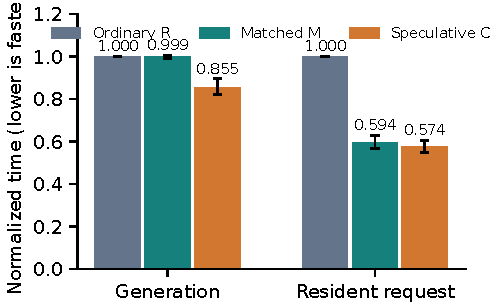
\includegraphics[width=0.62\linewidth]{figures/reference_cost.pdf}
\caption{RTX expansion costs normalized task-by-task to ordinary $R$, then geometrically averaged. Matched draft-free execution already reduces request cost substantially. Error bars invert the descriptive task-bootstrap intervals for $R/M$ and $R/C$. Bars are aggregate relative times, not additive cost components.}
\label{fig:reference}
\end{figure}

\begin{figure}[t]
\centering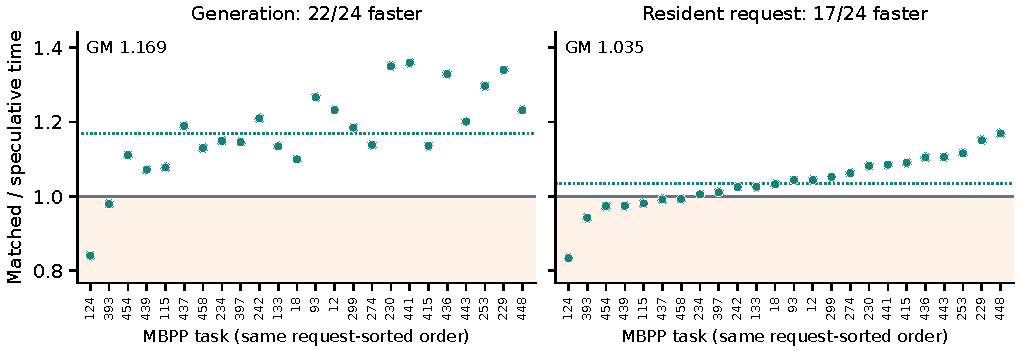
\includegraphics[width=0.96\textwidth]{figures/matched_task_effects.pdf}
\caption{RTX expansion: each point is the matched-target/candidate ratio of four-repetition absolute-time medians for one MBPP task. Both panels use the same order, sorted by request ratio. Generation improves on 22/24 tasks; resident-request time improves on 17/24. The line at one marks parity; the horizontal dotted line is the unweighted task geometric mean. Points are tasks, not independent repetitions.}
\label{fig:tasks}
\end{figure}

\subsection{Qualification and amortization boundaries}
Table~\ref{tab:boundary} summarizes the distinct outcomes. Passing the output gate does not imply passing the cost gate, and a failed output gate disqualifies a speed claim even if the recorded run is fast. The rows come from separate registered panels; they are not a pooled benchmark.
\begin{table}[t]
\centering\footnotesize\setlength{\tabcolsep}{3pt}
\caption{Observed qualification/cost combinations. Gen./req. speeds are against the named draft-free baseline; -- means no qualified speed claim.}
\label{tab:boundary}
\begin{tabular}{lccc}\toprule
Recipe & Qualified panel & Baseline & Gen./req.\\\midrule
RTX $k=3$, UB4 & 24 tasks & Matched & 1.169/1.035\\
RTX $k=7$, UB4 & 28 tasks & Matched & 0.997/0.950\\
RTX $k=7$, UB8 & Fails /229 & -- & --\\
B570 $k=2$ repair & 15 tasks & Ordinary & 0.283/0.201\\\bottomrule
\end{tabular}\end{table}
\subsection{Changing geometry can break the repair}
The expansion into draft length and microbatch capacity keeps failed cases. At paired $(k,\mathrm{UB})=(1,2)$ and $(3,4)$, the tested width/length panel qualifies. MBPP/229 fails at $(5,6)$ and $(7,8)$ under all measured cap contexts and repetitions, even though its wide ordinary and matched paths pass. The old HumanEval/18 probe also supplies an outside-panel failure at wider target-only capacity. Increasing the output cap does not certify every trajectory to that length: some responses finish much earlier, with observed maximum length 261 rather than a full 512-token stress trajectory.

A separate experiment holds UB4 fixed and tests $k=3,5,7$. All 28 exposed qualification tasks pass in two repetitions. The widest $k=7$ recipe is selected by qualification only, then measured in independent capture-off cost sessions. Against $k=3$, it obtains 0.82944$\times$ generation and 0.88987$\times$ request speed: qualified outputs, slower execution. Against matched target-only, $k=7$ reaches 0.99740$\times$ generation and 0.95035$\times$ request speed; the $k=3$ anchor reaches 1.20250$\times$ and 1.06797$\times$. Larger $k$ is neither a monotone correctness repair nor a monotone performance improvement in these contracts.

Diagnostic sessions, including warmup, record target caller calls falling from 305 to 199 while observed micrographs rise from 305 to 397. Separate formal work records show drafted tokens increasing from 3528 to 5392 and accepted tokens from 2772 to 3192. These are different sessions and must not be divided into one fabricated per-call measure. Micrograph observations are not CUDA kernel launches. The counts reveal why caller reduction is an inadequate performance proxy; they do not uniquely prove which component caused the slowdown. This limitation is consistent with prior work on verification cost~\cite{illusion}, while the fixed-capacity, reference-qualified counterexample adds a concrete numerical-contract boundary.

The resident serial-request study verifies reset behavior and positive finite costs on its own panel, approximately 1.181$\times$ generation and 1.039$\times$ request against its matched comparator. It is not a throughput or concurrency benchmark and is not pooled with the expansion.

\subsection{B570: repair without deployment gain}
The B570 frontend combines ordinary-reference prompt construction, in-place prefill-to-continuation phase binding from UB128 to UB1, and the existing $k=2$, draft-UB1 speculative loop. It qualifies 12 development requests, 112 requests over 56 exposed tasks, and all 30 candidate requests over 15 inputs unused in the accessible project. Qualification is the cap-128 endpoint contract from Section~\ref{sec:contracts}. The 30 candidate responses include extra raw suffix differences; endpoint equality cannot be rewritten as raw-array equality.

The formal E matrix is 119/120 complete because one old-N1 request lacks a payload. Ordinary $R$, matched target-only, and the candidate each have all 30 paid observations, so their 15 task-median pairs remain complete. Candidate speed is 0.28259$\times$ generation and 0.20129$\times$ request against ordinary $R$, slower in every paired round. Against matched target-only it is 0.28576$\times$ and 0.20570$\times$. Matched target-only itself is near the ordinary reference: 0.98889$\times$ and 0.97854$\times$. Thus the entire candidate regression cannot be attributed to a target consistency constraint alone.

Against 14 complete old-N1 task pairs, the candidate improves generation/request by 3.99309$\times$/2.63394$\times$, with a single request-round reversal at MBPP/245. This old-implementation improvement does not establish a deployable gain. Draft, accepted, caller and extra-suffix work are recorded, but no independent component profile identifies a unique remaining bottleneck. The measured recipe is a qualified cost failure; further optimization would require a different performance hypothesis.

\subsection{Global serialization as an earlier qualified cost failure}
An earlier RTX timing arm uses the same 19 exposed tasks as its prediction arm but 171 fresh observations: target-only UB1, batched speculation, and globally serialized speculation, each with three repetitions. Its direct-ID gate blocks batching at 51/57 arrays. Serialization qualifies at 57/57, yet its paired task-median speed is 0.677 times target-only, with descriptive interval [0.662,0.692] and zero of 19 prompts faster.

The global microbatch option also affects drafting. Its timer covers synchronized post-prefill work through slot release, including recorded sampler/state operations and logging. This is a different intervention and interval from the later attention-layout graph and server generation field. It cannot be combined with later results into a causal optimization trend. Its contribution is a separate qualified failure: global serialization preserved the tested reference but did not supply a useful latency operating point.

\subsection{Historical opportunities on M4 and 358H}
Historical M4 data supply a positive cost case. A prospective 60-task panel, 30 HumanEval plus 30 SpecBench~\cite{specbench} inputs, has three conditions and three repetitions: 540 requests. Fixed Always speculation and Guard each qualify 180/180 responses under that study's contract. Their post-prefill speedups against target-only are 1.34689$\times$ and 1.31139$\times$. Guard is 2.71\% slower than Always in geometric task latency. This guard has no measured advantage on the prospective panel.

A whole-request offline oracle choosing between target-only and Always by each observed task's medians improves on Always by only about 0.0692\% in geometric mean. It is a panel-specific choice oracle, not an upper bound for intra-request policies or other implementations. On Core Ultra 358H, CPU and NPU drafting reproduce the reference on their 90-request panels but yield 0.73392$\times$ and 0.35166$\times$ speed. Conditional removal of measured overhead leaves the available ceilings below parity. Full-prefix NPU replay and the historical target path are properties of that implementation, not impossibility results for heterogeneous decoding.


\subsection{Existing workload partitions reveal different operating points}
The fixed-UB width export separates 24 MBPP inputs and four HumanEval probes. Table~\ref{tab:strata} preserves these groups. At $k=7$, matched-target generation speed is 0.953 times on MBPP and 1.308 times on HumanEval; resident-request speed is 0.919 and 1.164 times. The pooled result is near generation parity and below request parity. Increasing width from $k=3$ remains slower in pooled costs, while the four-task HumanEval request result is approximately unchanged.

M4's separate prospective partition also has different gains: fixed speculation gives 1.570 times on HumanEval and 1.155 times on Spec-Bench. The guard reaches 1.555 and 1.106 times. The partitions illustrate why a global speed or accepted-token fraction does not specify which workload benefits. These are descriptive saved-data analyses, not a new adaptive method, validated routing rule, or CUDA/Metal comparison.
\begin{table}[t]\centering\footnotesize\setlength{\tabcolsep}{4pt}
\caption{Saved workload partitions. Speed is named baseline/candidate. RTX uses generation and resident-request timers; M4 uses its post-prefill timer. Rows are not cross-platform comparisons or independent validation panels.}
\label{tab:strata}
\begin{tabular}{llrlcc}\toprule
Study & Partition & Tasks & Comparison & Gen./post-prefill & Request\\\midrule
RTX width & MBPP & 24 & Anchor / wide & 0.806 & 0.873\\
RTX width & MBPP & 24 & Matched / wide & 0.953 & 0.919\\
RTX width & HumanEval & 4 & Anchor / wide & 0.985 & 1.000\\
RTX width & HumanEval & 4 & Matched / wide & 1.308 & 1.164\\
M4 & HumanEval & 30 & Target / fixed & 1.570 & --\\
M4 & HumanEval & 30 & Target / guard & 1.555 & --\\
M4 & Spec-Bench & 30 & Target / fixed & 1.155 & --\\
M4 & Spec-Bench & 30 & Target / guard & 1.106 & --\\
\bottomrule\end{tabular}\end{table}


\subsection{A target-work floor limits draft-only optimization}
The 358H measurements permit a conditional bound because complete target work was measured separately. For paired baseline cost $B_{ij}$ and target work $T_{ij}$, fixing progress and deleting all other nonnegative work implies
\begin{equation}
\operatorname{GM}_i\operatorname{median}_j S'_{ij}
\leq\operatorname{GM}_i\operatorname{median}_j(B_{ij}/T_{ij}).
\end{equation}
Prompt-estimator ceilings are 0.8372 times for CPU drafting and 0.8448 times for NPU drafting. Pooled-total ceilings differ: 0.8275 and 0.8352 times. Neither reaches parity. Even with other costs deleted, a uniform target-work reduction must reach at least 16.28\% or 15.52\% to make the prompt ceiling reach one. These are optimistic necessary budgets, not achieved improvements. Changed progress, target execution, or state interfaces require new qualification and measurement.
